The goal of this example was to complete a backward somersault, while maximizing the twist rotation.
The model is composed of a 6-DoF root segment and two 1-DoF torque actuated arms.
The OCP was solved for two models, the root rotations of the first one were expressed as euler rotations whereas they were expressed as a quaternion for the second one.
The movement lasted for approximately 1 second and was discretized using 100 shooting nodes.

Term $\#1$ of the objective function (Tab.~\ref{tab:Quaternion_base_twisting_somersault}) corresponds to maximizing the twist velocity and term $\#2$ is for control regularization.


\begin{table}[h!]
\caption{\small Objective terms of quaternion base maximally twisting somersault}
\label{tab:Quaternion_base_twisting_somersault}
\centering
\begin{tabular}{c c c c}
\toprule 
& Type & Function & Weight \\ 
\midrule
$\#1$ & Lagrange & MINIMIZE\_TWIST & $-1e1$ \\ 
\midrule
$\#2$ & Lagrange & MINIMIZE\_ TORQUE & $1e-6$ \\ 
\bottomrule
\end{tabular}
\end{table}


The solutions for both models were similar (Fig.~\ref{snapshots_quaternion_base_twisting_somersault}) highlighting the equivalence of the two rotation representations.
While euler angles have the advantage to be easily interpretable, they suffer from the loss of a DoF at the gimbal lock.
Therefore the use of quaternion representation is advantageous when a joint is free to rotate on a wide three-dimensional range for motion.


\begin{figure*}[t!]
\centering
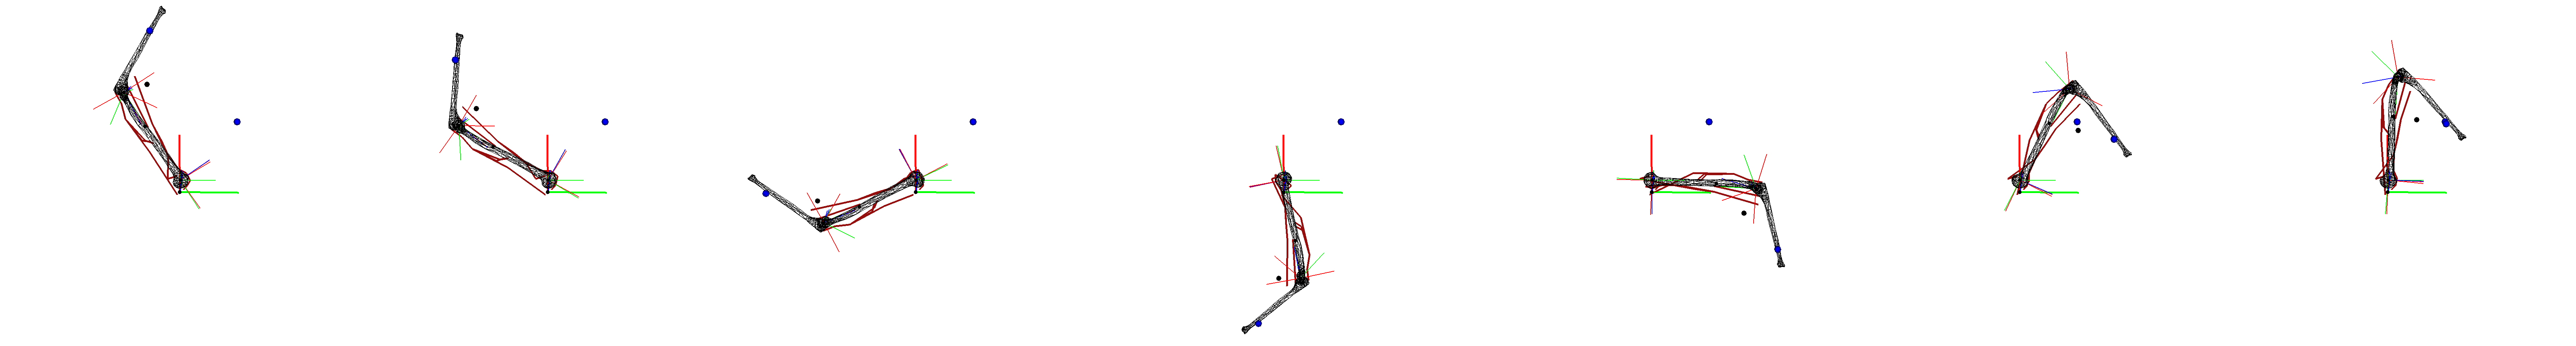
\includegraphics[width=\textwidth]{figures/activation_pointing_snapshots_acados.png}\\
\caption{Snapshots of a maximally twisting somersault driven by torque actuation. Top: euler angles. Bottom: quaternion. Changer la figure !!!!!!!!!!!!!!!!!!!!!!}
\label{fig:snapshots_quaternion_base_twisting_somersault}
\end{figure*}












